\documentclass[10pt,letterpaper]{article}
\usepackage[margin=1in]{geometry}
\usepackage[latin1]{inputenc}
\usepackage{amsmath}
\usepackage{amsfonts}
\usepackage{amssymb}
\usepackage{graphicx}
\usepackage{float}

\author{Roy Smart}
\begin{document}
	
	\noindent Hi Dana, \\
	
	I am still having a lot of trouble getting this hyperbolic heat conduction equation to work. Recall that we are trying to solve the system of equations
	\begin{gather}
		\tau + \frac{\partial q}{\partial t} + q = - \kappa \frac{\partial T}{\partial x} \\
		\frac{\partial T}{\partial t} = - \frac{\partial q}{\partial x},
	\end{gather}
	where we define the identity $c = \sqrt{\tau / \kappa}$. Using the Spitzer form of the conductivity, $\kappa = T^{5/2}$, and the Courant condition for hyperbolic differential equations, $c = f_{\text{CFL}} \Delta x / \Delta t$, we can write the damping coefficient as $\tau = \kappa / c^2 = T^{5/2}  [\Delta t^2 / (f_{\text{CFL}} \Delta x)]^2$. The timestep is given as some multiple ($\beta \approx 100$) of the parabolic timestep, $\Delta t = \beta \Delta t_{\text{diff}}$, where the parabolic timestep is $\Delta t_{\text{diff}} = f_{\text{CFL}} \Delta x^2 / (2 \kappa)$.
	
	Now, when I run my simulation, if I set $\beta = 1$, such that the hyperbolic and parabolic timesteps are the same, the differences between the parabolic and hyperbolic solutions are small (RMS error $\approx 10^{-5}$), which seems like the correct behavior. However, if I set $\beta$ to the smallest value described in Rempel 2017, $\beta=50$, the solution blows up, with large, nyquist-frequency oscillations starting in regions of high temperature and propagating across the entire domain (Figure \ref{b50}). This behavior occurs regardless of whether I've used a fully-explicit discretization of the system or the semi-implicit discretization that we discussed last week.	
	\begin{figure}[h]
		\centering
		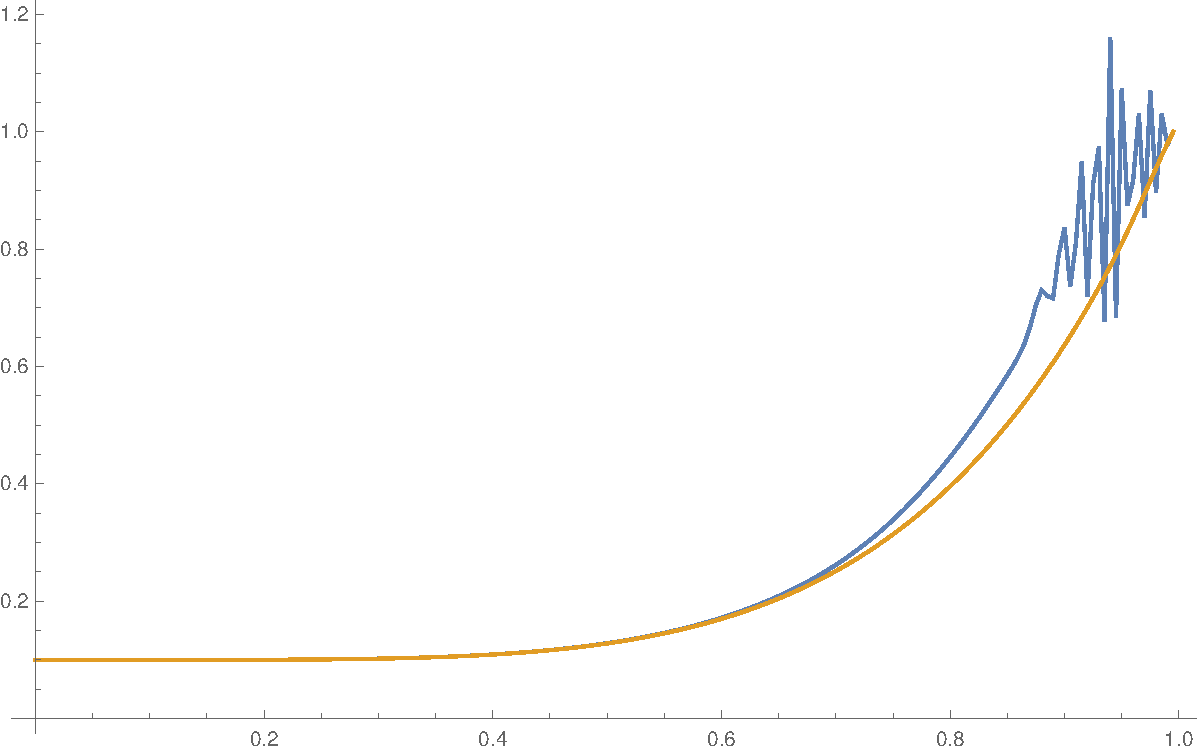
\includegraphics[width=0.5\textwidth]{b50_t125}
		\caption{Plot of the hyperbolic solution (blue) against the parabolic solution (orange) at timestep 125 (please note that the parabolic and hyperbolic solutions have different timestep sizes).}
		\label{b50}
	\end{figure}
	
	From this behavior, it would seem that $\tau$ needs to be smaller to \textit{increase} the damping, but making $\tau$ smaller only makes the problem worse, exploding much faster.  Making $\tau$ larger seems to stabilize the solution, however it becomes too wave-like, looking more like an oscillating string.
	
	Making $\kappa$ smaller also stabilizes the solution, but it just slows everything down such that the faster timestep is counteracted by the slower time-evolution. Making $\kappa$ larger destabilizes the solution.
	
	Ultimately, I feel as if I followed the procedure outlined in Rempel 2017 precisely and it doesn't work how he described it. Can you offer any hints as to why the solution isn't behaving as expected? Do you know of any debugging techniques that would be helpful to determine if the problem lies in my implementation? \\
	 
	 \noindent
	Thanks in advance for any advice that you can provide,\\
	Roy
	
\end{document}